\begin{center}
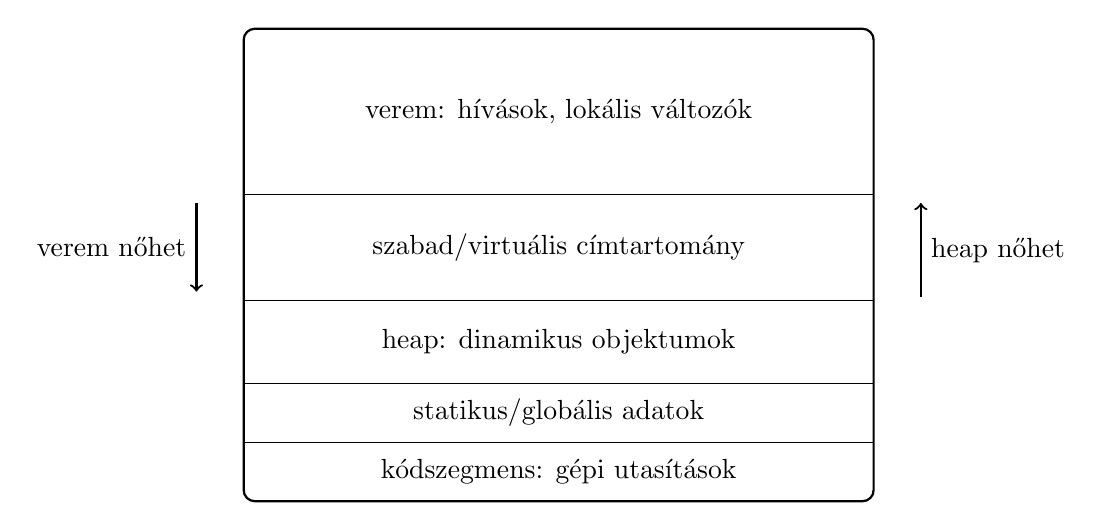
\begin{tikzpicture}[x=1cm,y=0.75cm]
  \draw[rounded corners, thick] (0,0) rectangle (8,8);
  \draw (0,1) -- (8,1);
  \draw (0,2) -- (8,2);
  \draw (0,3.4) -- (8,3.4);
  \draw (0,5.2) -- (8,5.2);
  \node at (4,0.5) {kódszegmens: gépi utasítások};
  \node at (4,1.5) {statikus/globális adatok};
  \node at (4,2.7) {heap: dinamikus objektumok};
  \node at (4,4.3) {szabad/virtuális címtartomány};
  \node at (4,6.6) {verem: hívások, lokális változók};
  \draw[->, thick] (8.6,3.45) -- (8.6,5.05) node[midway,right] {heap nőhet};
  \draw[->, thick] (-0.6,5.05) -- (-0.6,3.55) node[midway,left] {verem nőhet};
\end{tikzpicture}
\end{center}
